\newpage
\section{Suggested solutions: Frequency Response}


\begin{enumerate}
\item Consider an FIR filter approximation to the second derivative of the form
$$h[n]=T_{s}^{-2}\delta[n+1]-2T_{s}^{-2}\delta[n]+T_{s}^{-2}\delta[n-1].$$

\begin{enumerate}[a)]
\item The frequency response can be found by the DTFT (Equation \ref{eq:fresp_ct}) as
$$\mathcal{H}(\hat{\omega})=\sum_{k=-\infty}^{\infty}h[k]e^{-i\hat{\omega}k},$$
for this LTI system we get
$$\mathcal{H}(\hat{\omega})=T_{s}^{-2}e^{i\hat{\omega}}-2T_{s}^{-2}+T_{s}^{-2}e^{-i\hat{\omega}}=-2T_{s}^{-2}+T_{s}^{-2}2\cos(\hat{\omega})=\frac{2}{T_{s}^{2}}(\cos(\hat{\omega})-1).$$

\item The code shown in Listing \ref{code13_1} can be used to plot the spectral response. 
\begin{lstlisting}[language=Python, caption=Frequency response for finite difference,label=code13_1]
import numpy as n
import matplotlib.pyplot as plt

# plot in the principal spectrum (-pi,pi)
om = n.linspace(-n.pi,n.pi,num=1000)

# for simplicity take Ts as 1
Ts = 1

# definition of the frequency response function
def freq_resp(om):
    return 2/(Ts**2)*(n.cos(om)-1)

# plot the frequency response function over (-pi,pi)
plt.plot(om,n.abs(freq_resp(om)),label="$\mathcal{H}(\hat{\omega})$")
plt.legend()
plt.show()
\end{lstlisting}
Output of the code is shown in Figure \ref{spec_rep}.
\begin{marginfigure}
    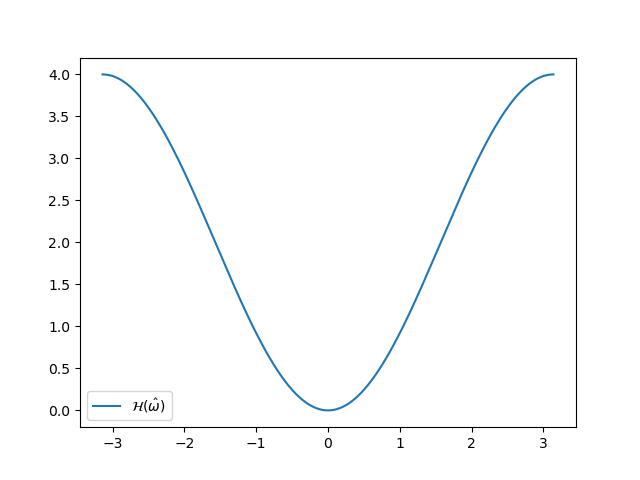
\includegraphics[width=7.0cm,height=6.5cm]{ch11/figures/freq13.png}
    \caption{Output of Listing \ref{code13_1}}
    \label{spec_rep}
\end{marginfigure}

\item In this case the frequency response function is real, so the phase response is $0$. Meaning there is no delay applied to the signal by this filter.

\item By looking at the plot of $|H(\hat{\omega})|$ we see that the filter is a high-pass filter as the frequencies around $0$ are greatly reduced. 

\item Inspecting the plot we see that for $\hat{\omega}=0$ the amplitude of the output signal will be $A'=0$. The reason is that in frequency domain we have
$$\hat{y}(\hat{\omega})=\mathcal{H}(\hat{\omega})\hat{x}(\hat{\omega}).$$

\item The phase is not changed by the filter so $\phi'=\phi$. For $\hat{\omega}=\pi/2$ the amplitude is doubled, so $A'=2A$, while for $\hat{\omega}=\pi$ the amplitude is scaled by $4$, giving $A'=4A$. This can be seen from the plot in Figure \ref{spec_rep} or by inserting the values into the frequency response function. 

\item The system $y(t)=\mathcal{T}\{x(t)\}=\frac{d^{2}}{dt^{2}}x(t)$ is a continuous-time LTI system, so
$$y(t)=\mathcal{H}(\omega)x(t).$$
In particular, if we take $x(t)=Ae^{i\phi}e^{i\omega t}$, then
$$y(t)=\frac{d^{2}}{dt^{2}}(Ae^{i\phi}e^{i\omega t})=Ae^{i\phi}(i\omega)^{2}e^{i\omega t}=-Ae^{i\phi}\omega^{2}e^{i\omega t}=-\omega^{2}(Ae^{i\phi}e^{i\omega t})=\mathcal{H}(\omega)x(t),$$
thus $\mathcal{H}(\omega)=-\omega^{2}$. 

\item Comparing the plots we conclude that the approximation is only good for small angular frequencies in the range $0<\omega<\pi/2$. 
\end{enumerate}

\item A running average filter is defined as
$$y[n]=\frac{1}{M}\sum_{k=0}^{M-1}x[n-k].$$
We'll assume that $M$ is an odd number. 

\begin{enumerate}[a)]
\item The impulse response function is obtained by feeding a Dirac-delta into the LTI system, so if $y[n]=\mathcal{T}\{x[n]\}$, then $h[n]=\mathcal{T}\{\delta[n]\}$. Doing this, we find that
$$\{h[n]\}_{n=0}^{M-1}=\frac{1}{M}.$$

\item The frequency response is the DTFT of $h[n]$, which gives
\begin{align*}
    \mathcal{H}(\hat{\omega})&=\sum_{k=0}^{M-1}\frac{1}{M}e^{-i\hat{\omega}k}=\frac{1-e^{-i\hat{\omega}M}}{M(1-e^{-i\hat{\omega}})}=\frac{1}{M}\left(\frac{e^{-i\hat{\omega}M/2}(e^{i\hat{\omega}M/2}-e^{-i\hat{\omega}M/2})}{e^{-i\hat{\omega}/2}(e^{i\hat{\omega}/2}-e^{-i\hat{\omega}/2})}\right) \\
    &=\underbrace{\frac{1}{M}\frac{\sin(\hat{\omega}M/2)}{\sin(\hat{\omega}/2)}}_{D_{M}(\hat{\omega})}e^{-i\hat{\omega}(M-1)/2}.
\end{align*}
The sum is evaluated using known formulas for geometric sums. 

\item If we have a system with impulse response $h_{\tau}[n]=\delta[n-\tau]$, then the frequency response is
$$\mathcal{H}_{\tau}(\hat{\omega})=\sum_{k=-\infty}^{\infty}h[k]e^{-i\hat{\omega}k}=\sum_{k=-\infty}^{\infty}\delta[k-\tau]e^{-i\hat{\omega}k}=e^{-i\hat{\omega}\tau}.$$

\item The following code can be used to make the plot shown in \ref{freq_responses}
\begin{lstlisting}[language=Python, caption=Plotting the frequency response code,label=code14_2]
import numpy as n
import matplotlib.pyplot as plt
import scipy.special as dd

# partition the interval (-pi,pi)
om = n.linspace(-n.pi,n.pi,num=1000)

# use M = 11 for the Dirichlet kernel plot
M = 11

# plot the two functions in the same coordinate system
plt.plot(om,n.abs(dd.diric(om,n=M))**2,label="$|D_{11}(\hat{\omega})|^{2}$")
plt.plot(om,n.abs(n.exp(1j*om*(M-1)/2)*dd.diric(om,n=M))**2,label="$|H_{11}(\hat{\omega})|^{2}$")
plt.xlabel("$\hat{\omega}$")
plt.legend()
plt.show()
\end{lstlisting}
As expected the functions are identical. 
\begin{marginfigure}
    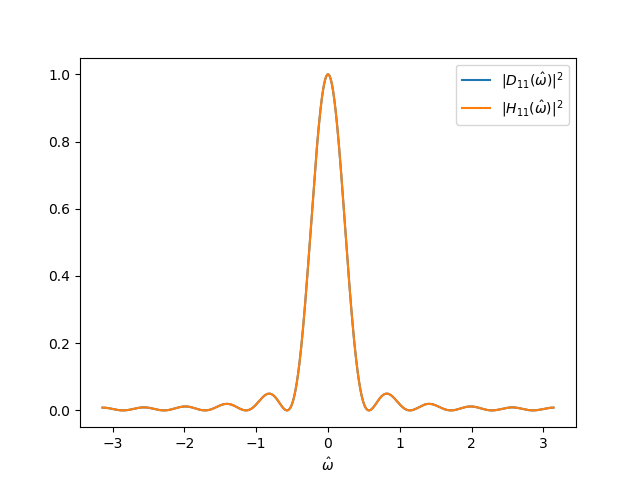
\includegraphics[height=7.0cm,width=7.5cm]{ch11/figures/frequency_responses.png}
    \caption{Comparison of frequency responses}
    \label{freq_responses}
\end{marginfigure}

\item The frequency response function was derived in b), and it has the form 
$$\mathcal{H}(\hat{\omega})=D_{M}(\hat{\omega})\mathcal{H}_{\tau}(\hat{\omega}),$$
where $\mathcal{H}_{\tau}(\hat{\omega})$ is a time-shift system with $\tau=(M-1)/2$. 

\item Claim: $|\mathcal{H}(\hat{\omega})|^{2}=|D_{M}(\hat{\omega})|^{2}$.
\begin{proof}
A simple computation gives
\begin{align*}
    |\mathcal{H}(\hat{\omega})|^{2}&=\mathcal{H}(\hat{\omega})\mathcal{H}^{*}=(\hat{\omega})(D_{M}(\hat{\omega})\mathcal{H}_{\tau}(\hat{\omega}))(D_{M}(\hat{\omega})\mathcal{H}_{\tau}(\hat{\omega}))^{*}\\
    &=|D_{M}(\hat{\omega})|^{2}e^{-i\hat{\omega}\tau}e^{i\hat{\omega}\tau}=|D_{M}(\hat{\omega})|^{2},
\end{align*}
as claimed. 
\end{proof}
In conclusion the running average filters produce the same magnitude response, but one of them induces a time-shift while the other doesn't. 
\end{enumerate}



\end{enumerate}


